\documentclass[12pt]{article}
\usepackage{amsmath}
\usepackage{amssymb}
\usepackage{geometry}
\usepackage{enumerate}
\usepackage{natbib}
\usepackage{float}%稳定图片位置
\usepackage{graphicx}%画图
\usepackage[english]{babel}
\usepackage{a4wide}
\usepackage{indentfirst}%缩进
\usepackage{enumerate}%加序号
\usepackage{mathabx}%积分
\usepackage{multirow}%合并行
\title{\large UM-SJTU JOINT INSTITUTE\\Intro to Circuits\\(VE215)\\\ \\\ \\\ \\\ \\\ \\\ \\\ \\\ \\\ \\\ \\\
LABORATORY REPORT\\\ \\\ EXERCISE 4\\\ AC Lab \\\ \\\ \\\ \\\ \\\ }
\author{Name: Pan Chongdan\\ID: 516370910121}
\date{Date: \today}
\begin{document}
\maketitle
\newpage
\section{Introduction and Theoretical Background}
\subsection{Objectives}
\begin{enumerate}
\item Define, calculate and measure the amplitude of a sinusoidal signal.
\item Define, calculate and measure the rise time and fall time of a signal.
\item Observe FFT spectra of signal and measure their parameters with cursors.
\item Measure the waveform and FFT spectra of various signal
\item Compare the theoretical results and the results obtained in the lab word.
\end{enumerate}
\subsection{Introduction}
\subsubsection{High-Z Mode}
The function generator is like a Thevenin circuit including a voltage source $V_S$ and a equivalent resistance of 50$\Omega$.
\begin{figure}[H]
\centering
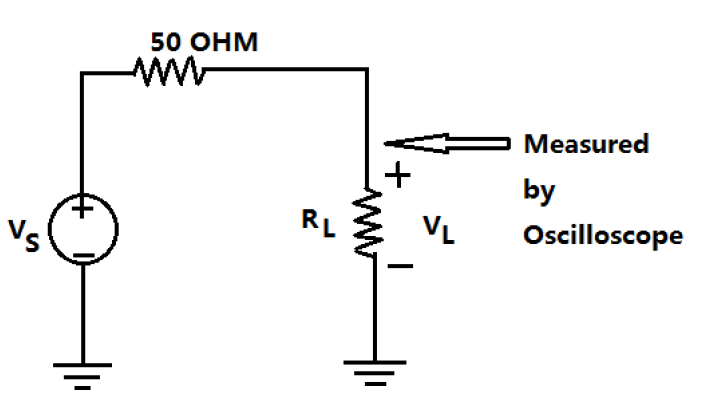
\includegraphics[scale=0.5]{P1.jpg}
\end{figure} 
\par When $R_L=50\Omega$, according to voltage division, $V_L$ is 0.5 $V_S$. If 2$V_{ppk}$ is set for the function generator, the actual $V_S$ will be 4$V_{ppk}$ to make sure the load get a voltage of $2V_{ppk}$.
\par In the lab work, the load resistance $R_L$ is about $1M\Omega$, so the $V_L$ measured across $R_L$ practically equals $V_S$. In the High-Z mode.the function generator will produce voltage $V_S$ and display it. 
\subsection{The Rise Time and Fall Time of Signals}
The Rise time is the interval between the moment of the time when the signal reaches the $10\%$ level and the moment of time when it reaches $90\%$ level.
\begin{figure}[H]
\centering
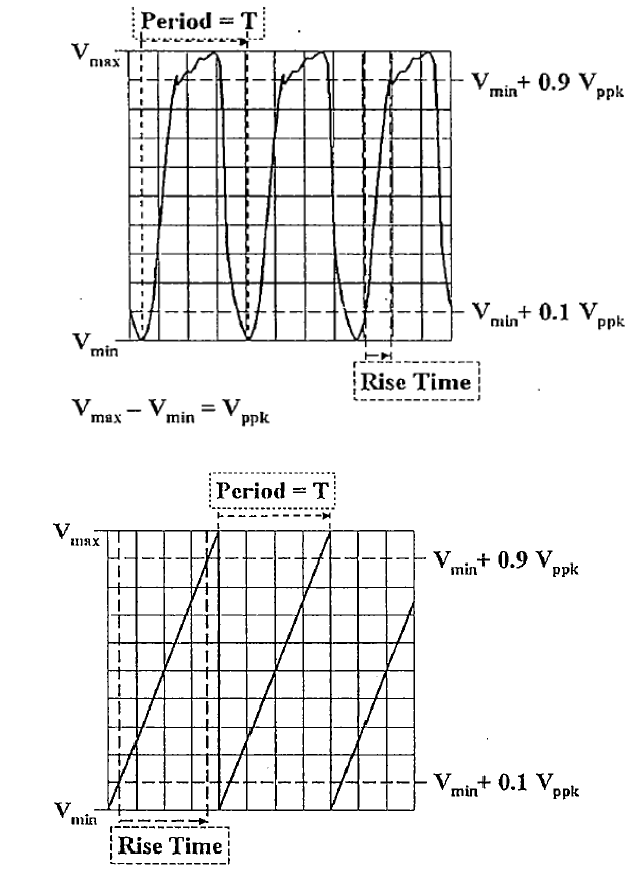
\includegraphics[scale=0.5]{P2.jpg}
\end{figure} 
\par The above two figures illustrate the rise time of a sinusoidal like wave and a saw-tooth wave.Take the sinusoidal wave as an example to calculate the rise time:
$$y=\frac{V_{ppk}}{2}sin(2\pi ft)$$
$$V_{min}=\frac{-V_{ppk}}{2},V_{max}=\frac{-V_{ppk}}{2}$$
$$RiseTime=\frac{sin^{-1}(\frac{V_{min}+0.9V_{ppk}}{0.5V_{ppk}})-sin^{-1}(\frac{V_{min}+0.1V_{ppk}}{0.5V_{ppk}})}{2\pi f}$$
\subsection{Fourier Series Representation of a Signal}
Fourier series is a way to represent a wave-like function as a combination of
simply sine waves. It decomposed and period function into the sum of a set of simple oscillation functions.
\par Let $(x)$ be a periodic signal with fundamental period $T_0$. It can be represented by the following synthesis equation 
$$x(t)=\sum_{k=-\infty}^{\infty}c_ke^{jk\omega_0t}(\omega=\frac{2\pi}{T_0})$$
The coefficient $c_k$ in the above equation can be calculated by the analysis equation
$$c_k=\frac{1}{T_0}\int^{T_0}_0x(t)e^{-jk\omega_0t}dt,k=0,\pm1,\cdots$$
\par for Mathematic code:
\begin{figure}[H]
\centering
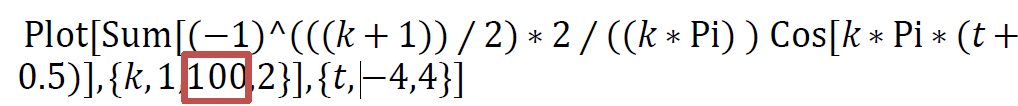
\includegraphics[scale=0.3]{P3.jpg}
\end{figure}
The larger the value in red box is, the more accurate the figure will be.
\begin{figure}[H]
\centering
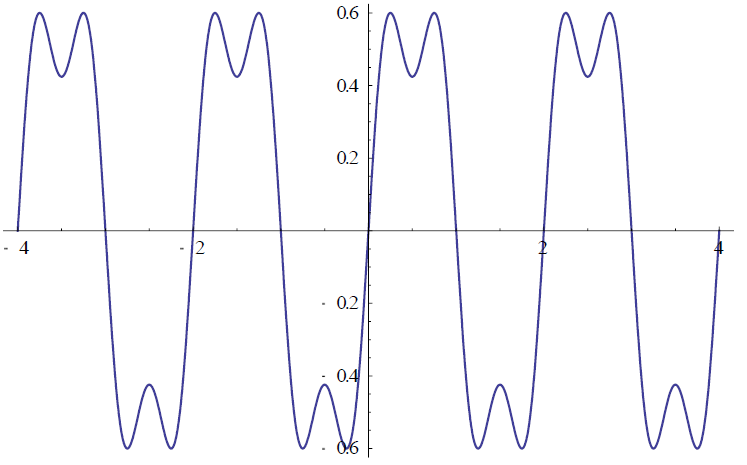
\includegraphics[scale=0.3]{P4.jpg}
\caption{For value 3}
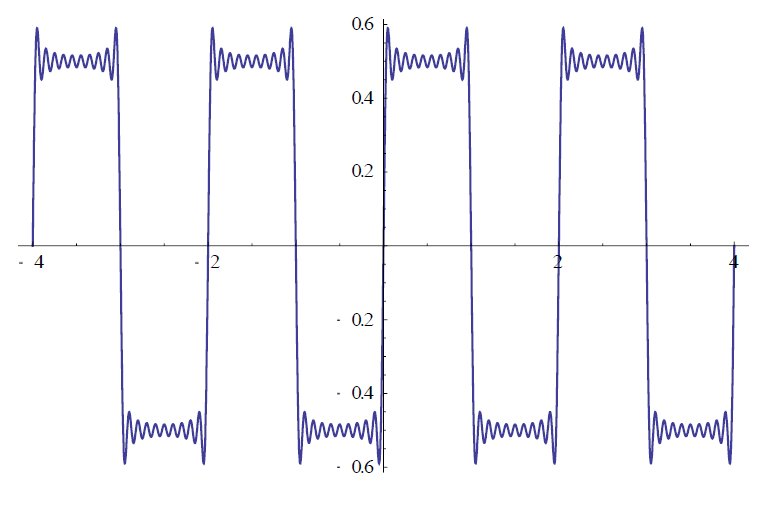
\includegraphics[scale=0.3]{P5.jpg}
\caption{For value 20}
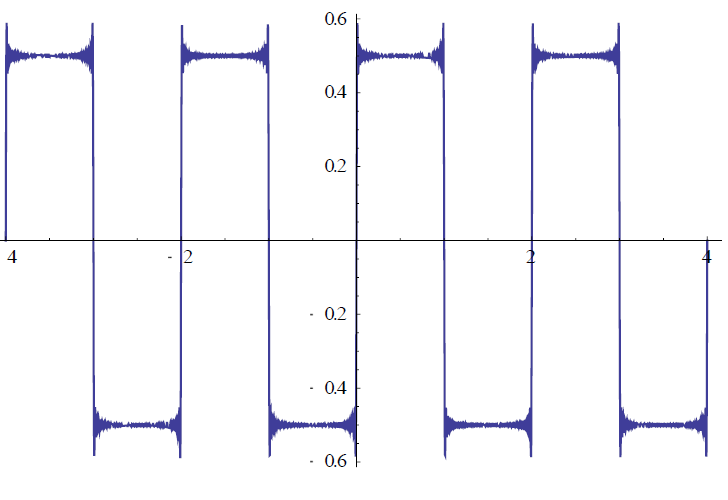
\includegraphics[scale=0.3]{P6.jpg}
\caption{For value 100}
\end{figure}
\subsection{Four ways to measure the amplitude of a sinusoid}
\begin{enumerate}
\item $V_{peak}=V_p=V_{pk}=V_0$ is the peak amplitude of the sinusoid measured in V or mV.
\item $V_{ppk}=V_{max}-V_{min}=2V_0$ is the value we often use in the lab to determine the overall size of the waveform, We've used it many times in the previous labs.
\item $V_{RMS}$ is the Root-Mean-Square, or RMS amplitude of the sinusoid. The sinusoid voltage $V=V_0sin(\omega t+\theta)$ dissipates as much power in the load resistor as does the DC voltage equals to $V_{RMS}$.
\begin{figure}[H]
\centering
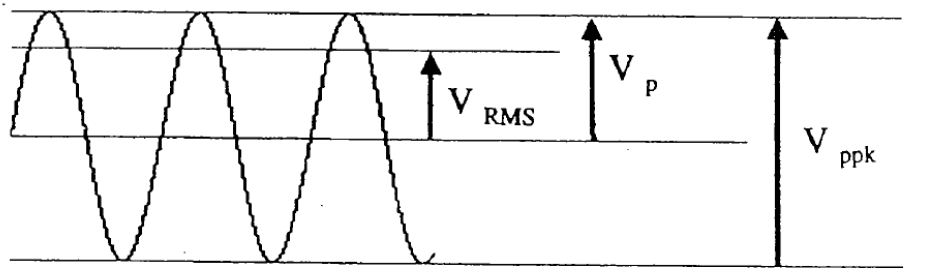
\includegraphics[scale=0.4]{P7.jpg}
\end{figure}
For any periodic function $f(t)$ that has period $T$, the RMS amplitude is defined as
$$Amplitude,RMS=\sqrt{\frac{1}{T}\int^{t_0+T}_{t_0}(f(t))^2dt}$$
In the case of sinusoid $f(t)=V_0sin(\omega t+\theta)$
$$V_{RMS}=\frac{V_0}{\sqrt{2}}=\frac{V_{peak}}{\sqrt{2}}=\frac{V_{ppk}}{2\sqrt{2}}$$
\item The above three ways all study the signal in time domain, plotted as voltage vs.
time. We also study the frequency domain by measuring their spectra displayed as amplitude vs. frequency. In frequency domain, the oscilloscope measures the amplitude of on a logarithmic scale, using decibels.
$$AmplitudeInDecibels(dBV)=20\cdot log_{10}(\frac{AmplitudeInV_{RMS}}{1V_{RMS}})$$
Decibels are used to calculate ratios of two amplitudes on a logarithmic scale.
$$RatioInDecibels(dB)=20\cdot log_{10}(\frac{Signal\#2'sAmplitude,RMS}{Signal\#1'sAmplitude,RMS})$$
\end{enumerate}
\section{Procedure}
\subsection{Part 1}
\begin{enumerate}
\item I set a sine wave at 1 [kHz] and keep its amplitude at 3 [Vpp] on the function generator. The load must be High-Z mode.
\item I record the parameters and fill the table with the data set on the function generator and displayed on the oscilloscope.
\item I repeat the Step 2 with a sine wave at 1.5 [kHz] and 5 [Vpp] on the function
generator. The load should remain High-Z mode.
\item I calculate the rise time in theory and compare it with the values displayed.
\end{enumerate}
\subsection{Part 2}
\begin{enumerate}
\item I set a sine wave and a square wave, respectively. The frequency is 1
[kHz] and the amplitude is 3 [Vpp].
\item I set 1 [V/div] and 5 [ms/div] on the oscilloscope.
\item I push the “MATH” button and select “FFT” function. Push the “cursor” button and select “trace” mode to trace the spectrum.
\item When the cursor reach a peak of the spectrum, I record the Frequency in [kHz]
and the Amplitude in [dBV].
\item I Set another sine wave and a square wave with the frequency is 2 [kHz] and the
amplitude is 6 [Vpp], then I repeat the steps above.
\item I calculate theoretical amplitude of sine wave in [dBV] and the $V_{peak}$ of each square wave
measured in Part II
\end{enumerate}
\section{Results}
\subsection{Part 1}
\begin{table}[H]
\centering
\begin{tabular}{|c|c|c|}
\hline
                & Set on Function Generator & Measured with Oscilloscope \\ \hline
Amplitude in $V_{pp}$ [V]   & 3.000                     & 3.100                      \\ \hline
Frequency [kHz] & 1.000                     & 1.005                      \\ \hline
Rise Time [$\mu s$]      & 295.17                    & 276.58                     \\ \hline
Amplitude in $V_{pp}$ [V]    & 5.000                     & 5.01                       \\ \hline
Frequency [kHz] & 1.500                     & 1.4996                     \\ \hline
Rise Time [$\mu s$]      & 196.78                    & 184.95                     \\ \hline
\end{tabular}
\caption{Rise Time Measurement}
\end{table}
\subsection{Part 2}
\begin{enumerate}
\item Set the wave at 3[$V_{pp}$] 1[kHz]
\begin{table}[H]
\centering
\begin{tabular}{|c|c|c|}
\hline
Peak  & Frequency (measured) [kHz] & Amplitude (measured) [dBV] \\ \hline
$f_0$ & 1.000                      & -0.261                     \\ \hline
\end{tabular}
\caption{FFT spectrum for Sine Wave}
\end{table}
\begin{table}[H]
\centering
\begin{tabular}{|c|c|c|}
\hline
Peak  & Frequency (measured) [kHz] & Amplitude (measured) [dBV] \\ \hline
$f_0$ &1.000  &-1.878  \\ \hline
$3f_0$ &3.000  &-7.790  \\ \hline
$5f_0$ &5.001  &-12.519  \\ \hline
$7f_0$ &7.003  &-15.520  \\ \hline
$9f_0$ &9.001  &-17.516  \\ \hline
\end{tabular}
\caption{FFT spectrum for Square Wave}
\end{table}
\item Set the wave at 6[$V_{pp}$] 2[kHz]
\begin{table}
\centering
\begin{tabular}{|c|c|c|}
\hline
Peak  & Frequency (measured) [kHz] & Amplitude (measured) [dBV] \\ \hline
$f_0$ & 1.999                      & 5.494                     \\ \hline
\end{tabular}
\caption{FFT spectrum for Sine Wave}
\end{table}
\begin{table}[H]
\centering
\begin{tabular}{|c|c|c|}
\hline
Peak  & Frequency (measured) [kHz] & Amplitude (measured) [dBV] \\ \hline
$f_0$ &2.000  &7.658  \\ \hline
$3f_0$ &6.001  &-2.006  \\ \hline
$5f_0$ &10.000  &-6.527  \\ \hline
$7f_0$ &14.000  &-9.169  \\ \hline
$9f_0$ &18.000  &-11.650  \\ \hline
\end{tabular}
\caption{FFT spectrum for Square Wave}
\end{table}
\end{enumerate}
\section{Conclusion}
\subsection{Part 1}
In first part of the lab, I set a sine wave on the function generator and record its amplitude, frequency, and rise time. When the amplitude is $3V_{pp}$ and frequency is 1kHz, the rise time measured on the function generator and oscilloscope are 295.17$\mu s$ and $276.58\mu s$, which is very close to my theoretical data 295$\mu s$.
$$RiseTime=\frac{sin^{-1}(\frac{V_{min}+0.9V_{ppk}}{0.5\cdot3})-sin^{-1}(\frac{V_{min}+0.1V_{ppk}}{0.5\cdot3})}{2000\pi}=295[\mu s]$$
\par Then I change the amplitude to 5$V_{pp}$ and frequency to 1.5, the rise time is measured as 196.78$\mu s$ and 184.95$\mu s$,while my calculated data is 196.7$\mu s$.
$$RiseTime=\frac{sin^{-1}(\frac{V_{min}+0.9V_{ppk}}{0.5\cdot6})-sin^{-1}(\frac{V_{min}+0.1V_{ppk}}{0.5\cdot6})}{2000\pi}=196.7[\mu s]$$
\par My calculated data is the same as it on the function generator but the data on the oscilloscope is a bit smaller than it.
\subsection{Part 2}
In the second par of the lab, I measured the frequency and amplitude in dBV of since and square wave of different amplitude in $V_{pp}$ and frequency. 
\par When the amplitude of the sine wave is 3$V_{pp}$, my calculated amplitude in dBV is 0.512, which is bigger than my measured value -0.261.
\par When the amplitude of the sine wave is 6$V_{pp}$, my calculated amplitude in dBV is 6.532, which is also bigger than my measured value 5.494.
\par For the square wave, my calculated value is always bigger than the measured data.
$$v=20log\frac{3\sqrt{2}}{\pi\cdot(2n-1)}$$
$$v_1=20log\frac{3\sqrt{2}}{\pi}=2.610$$
\begin{table}[H]
\centering
\begin{tabular}{|c|c|c|}
\hline
Peak & Measured Amplitude in dBV & Calculated Amplitude in dBV \\ \hline
$f_0$      & 1.878                          & 2.610                            \\ \hline
$3f_0$     & -7.970                          &-6.932                             \\ \hline
$5f_0$     & -12.519                          &-11.370                             \\ \hline
$7f_0$     & -15.520                          &-14.292                             \\ \hline
$9f_0$     & -17.516                          &-16.475                             \\ \hline
\end{tabular}
\caption{Amplitude when the square wave is set at 3[$V_{pp}$] 1 kHz}
\end{table}
\begin{table}[H]
\centering
\begin{tabular}{|c|c|c|}
\hline
Peak & Measured Amplitude in dBV & Calculated Amplitude in dBV \\ \hline
$f_0$      & 7.658                          & 8.630                            \\ \hline
$3f_0$     & -2.006                          &-0.912                             \\ \hline
$5f_0$     & -6.527                          &-5.349                             \\ \hline
$7f_0$     & -9.169                          &-8.271                             \\ \hline
$9f_0$     & -11.650                          &-10.455                             \\ \hline
\end{tabular}
\caption{Amplitude when the square wave is set at 6[$V_{pp}$] 2 kHz}
\end{table}
In this lab, I learned about the principle of High-Z mode of the function generator and reviewed the concept of rise time and fall time of signals. Also, I had a general idea about the Fourier Series and how to use it to represent a square wave signal. In addition, I learned four ways to calculate amplitude of a sinusoid in $V_{peak},V_{ppk},V_{RMS},$ and in dBV. I calculate the amplitude in dBV of square and sinusoid wave at different amplitude and frequency and compared it with the data measured in the lab work.
\section{Reference}
\begin{enumerate}[-]
\item \emph{VE215FA2017 AC LabManual} 
\item \emph{Circuits Make Sense}, Alexander Ganago, Department of Electrical Engineering and Computer Science, University of Michigan, Ann Arbor.
\end{enumerate}
\end{document}